\documentclass[12pt]{article}

% Packages
\usepackage[margin=1in]{geometry}
\usepackage{amsmath, amssymb}
\usepackage{graphicx}
\usepackage{float}
\usepackage{caption}
\usepackage{hyperref}
\usepackage[most]{tcolorbox}
\emergencystretch = 2em

\setlength{\parindent}{0pt}

% Title Information
\title{Principles of Feedback Control Project}
\author{Wesley Hon \\ EC ENGR 141 \\ Professor Xiaofan Cui}
\date{March 15th, 2026}

\begin{document}

\maketitle

\begin{abstract}
This project analyzes and controls a DC power system supplying a constant power load (CPL) through an L-R-C network. The system is first modeled using nonlinear state-space equations with the inductor current and capacitor voltage selected as the state variables. The nonlinear dynamics arise from the constant power load, which introduces a nonlinear current term proportional to $\dfrac{P}{v_{DC}}$. The model is then linearized around an equilibrium operating point to obtain a linear state-space representation. From this linearized model, the transfer function relating the input voltage perturbation to the output capacitor is derived and the stability of the system is analyzed. \\

Using the obtained linear model, a controller is then designed and implemented in Simulink to meet specified time-domain requirements, including a settling time of less than 0.05s and no overshoot. The controller is first tested on the linearized system and then applied to the original nonlinear system while enforcing physical safety constraints through saturation limits on voltage and current. Simulation results demonstrate the behavior of the controlled system and show differences between the linearized and nonlinear models. The results illustrate the destabilizing effects of constant power loads and the importance of appropriate controller design for maintaining stability in DC power systems. 
\end{abstract}

\newpage

\tableofcontents

\begin{center}
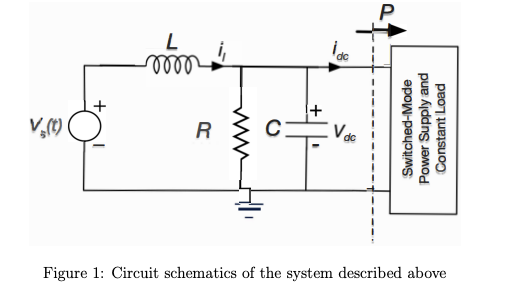
\includegraphics[width = 0.7\textwidth]{lrc.png}
\end{center}

\newpage

\Large{Defining the Physical System}\\

\large{Circuit Components}\\
\normalsize{}
\begin{tcolorbox}[enhanced, frame hidden, colback=white, borderline west={1pt}{0pt}{gray}]
\begin{minipage}{0.5\textwidth}
  \begin{align*}
    V_s(t) & & \text{(DC source input)}\\
    L & & \text{(Inductor)}\\
    C & & \text{(Capacitor)}\\
    R & & \text{(Parallel Resistor)}\\
   \text{Cosntant Power Load (CPL)} & & \text{modeled as power P}\\
  \end{align*}
\end{minipage}
\end{tcolorbox}

\

\large{States}
\normalsize{}
\begin{tcolorbox}[enhanced, frame hidden, colback=white, borderline west={1pt}{0pt}{gray}]
Capacitor node voltage: $v_{dc}$\\
Inductor current: ${i_l}$\\
$\hookrightarrow$ states of the system.
\end{tcolorbox}

\

\large{CPL}
\normalsize{}
\begin{tcolorbox}[enhanced, frame hidden, colback=white, borderline west={1pt}{0pt}{gray}]
CPL draws constant power. No constant resistance.\\

Power relation: $P = v_{dc} * i_{dc}$\\

Thus, $i_{dc} = \dfrac{P}{v_{dc}}$\\

The system is nonlinear.
\end{tcolorbox}

\

\large{State Variables}
\normalsize{}
\begin{tcolorbox}[enhanced, frame hidden, colback=white, borderline west={1pt}{0pt}{gray}]
  \begin{tcolorbox}[enhanced, frame hidden, colback=white, borderline west={1pt}{0pt}{gray}]
    \begin{align*}
      x_1(t) &= i_l(t)\\
      x_2(t) &= v_{dc}(t)\\
    \end{align*}
  \end{tcolorbox}
  Input: $u(t) = v_s(t)$\\
  Output: $y = v_{dc}$
\end{tcolorbox}


\newpage 

\section{State-Space Representation of the System}
Considering the inductor current and the capacitor voltage as your two states (i.e., $x_1(t) = i_1(t)$ and $x_2(t) = v_{dc}(t)$), obtain the state-space representation for this system in the form of $\dot{x} = f(x, u)$ where $u(t) = v_s(t)$. Recall that power supplied to the load is the product of the current through and the voltage across it.\\

\textbf{Goal:} Solve for the state space representation of the system in the form $\dot{x} = f(x, u)$.\\

Analyzing the circuit, the circuit components are one inductor (L) in series and two branches of a resistor and a capacitor (C) down to ground. \\

\begin{tcolorbox}[enhanced, frame hidden, colback=white, borderline west={1pt}{0pt}{gray}]
  \large{$\dot{x_1}$ through the voltage across the inductor}
  \normalsize{}
  \begin{align*}
    L\dfrac{di_l}{dt} &= v_s - v_{dc} & \ & \text{voltage across the inductor}\\
    \dot{x_1} &= \dfrac{1}{L}(v_s-v_{dc}) & \ & \text{where } x_1 = i_l
  \end{align*}
\end{tcolorbox}

\

\begin{tcolorbox}[enhanced, frame hidden, colback=white, borderline west={1pt}{0pt}{gray}]
  \large{$\dot{x_2}$ through the voltage across the capacitor}
  \normalsize{}
  \begin{align*}
    C\dfrac{dv_{dc}}{dt} &= i_l - i_R -i_{dc} & \ & \text{current through the capacitor}
  \end{align*}
  \begin{tcolorbox}[enhanced, frame hidden, colback=white, borderline west={1pt}{0pt}{gray}]
    Resistor current: \ $i_R = \dfrac{v_{dc}}{R}$\\
    CPL current: \ $i_{dc} = \dfrac{P}{v_{dc}}$
  \end{tcolorbox}
  \begin{align*}
    C\dfrac{dv_{dc}}{dt} &= i_l - \dfrac{v_{dc}}{R} -\dfrac{P}{v_{dc}} & \ & \text{sub the currents}\\
    \dot{x_2} &= \dfrac{1}{C}(i_l - \dfrac{v_{dc}}{R} -\dfrac{P}{v_{dc}}) & \ & \text{where } x_2 = v_{dc}
  \end{align*}
\end{tcolorbox}

\

\begin{tcolorbox}[enhanced, frame hidden, colback=white, borderline west={1pt}{0pt}{gray}]
  \large{Nonlinear Model -- State Space Representation of the System}
  \normalsize{}
  \[
  \boxed{
    \begin{aligned}
      \dot{x_1} &= \dfrac{1}{L}(v_s - x_2)\\
      \dot{x_2} &= \dfrac{1}{C}(x_1 - \dfrac{x_2}{R} - \dfrac{P}{x_2})\\
    \end{aligned}
  }
  \]

  where:\\
  $\hookrightarrow$ $x_1 = i_l(t)$\\
  $\hookrightarrow$ $x_2 = v_{dc}(t)$
\end{tcolorbox}

\

\begin{tcolorbox}[enhanced, frame hidden, colback=white, borderline west={1pt}{0pt}{gray}]
  \begin{minipage}[t]{0.6\textwidth}
    \vspace{0pt}
    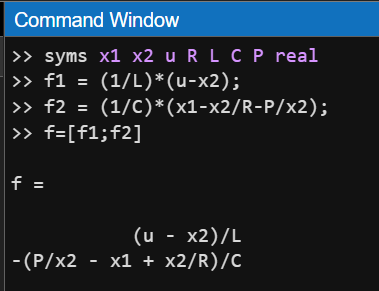
\includegraphics[width = \textwidth]{matlab1.png}
  \end{minipage}\hfill
  \begin{minipage}[t]{0.35\textwidth}
    \vspace{5pt}
    \textbf{Code Snippet 1}:
    This MATLAB script shows the creation of the variables $x_1, x_2, u, R, L, C, P$. It defines $f_1$ and $f_2$ as variables for the state space representation $\dot{x_1}$ and $\dot{x_2}$ respectively. Additionally printing $f$ as the matrix of the state space representation of the system.
  \end{minipage}
\end{tcolorbox}

\

\section{Linearized Dynamics}
Assume that the system has an equilibrium point at $(i_{l_0}, v_{dc_0}, v_{s_0})$. Obtain the linearized dynamics of this system in the form of $\delta\dot{x} = A\delta x + B\delta u$ where $\delta x \triangleq [i_l - i_{l0} \;\; v_{dc} - v_{dc0}]^{T}$ and $\delta u \triangleq v_s - v_{s0}$. Find matrices A and B.\\

\textbf{Goal:} Get the linearized dynamics of the system in the form of $\delta\dot{x} = A\delta x + B\delta u$ and find the matrices A and B.\\

\begin{tcolorbox}[enhanced, frame hidden, colback=white, borderline west={1pt}{0pt}{gray}]
  Linearize around the equilibrium: $(i_{l0}, v_{dc0}, v_{s0})$
  \begin{tcolorbox}[enhanced, frame hidden, colback=white, borderline west={1pt}{0pt}{gray}]
    Deviations:
    \begin{align*}
      \delta x &= \begin{bmatrix}
        i_l - i_{i0}\\
        v_{dc} - v_{dc0}\\
      \end{bmatrix}\\
      \delta u &= v_s - v_{s0}
    \end{align*}
  \end{tcolorbox}
  Linear system form: $\delta \dot{x} = A \delta x + B \delta u$\\
  Deviations from the equilibrium point is given by a deviation in $x$ and a deviation in $u$ that causes a total deviation in the system $\dot{x}$.
\end{tcolorbox}

\

\begin{tcolorbox}[enhanced, frame hidden, colback=white, borderline west={1pt}{0pt}{gray}]
  \large{Matrix A}\\
  \normalsize{}
  Partial derivative of $f(x, u)$\\
  \begin{minipage}{0.4\textwidth}
    \begin{align*}
      &\text{First Equation:} &\\
      &&\dot{x_1} &= \dfrac{1}{L}(v_s - x_2)\\
      &\text{Derivatives:}&\\
      &&\dfrac{\partial}{\partial x_1} &= 0\\
      &&\dfrac{\partial}{\partial x_2} &= -\dfrac{1}{L}\\
    \end{align*}
  \end{minipage}
  \begin{minipage}{0.04\textwidth}
    \
  \end{minipage}
  \begin{minipage}{0.4\textwidth}
    \begin{align*}
      &\text{Second Equation:} &\\
      &&\dot{x_2} &= \dfrac{1}{C}(x_1 - \dfrac{x_2}{R} - \dfrac{P}{x_2})\\
      &\text{Derivatives:}&\\
      &&\dfrac{\partial}{\partial x_1} &= \dfrac{1}{C}\\
      &&\dfrac{\partial}{\partial x_2} &= \dfrac{1}{C}(-\dfrac{1}{R} + \dfrac{P}{v^2_{dc0}})\\
    \end{align*}
  \end{minipage}
  Thus,\\
  \[
    \boxed{
      A =
      \begin{bmatrix}
        0 & -\dfrac{1}{L}\\
        \dfrac{1}{C} & \dfrac{1}{C}(-\dfrac{1}{R} + \dfrac{P}{v^2_{dc0}})\\
      \end{bmatrix}
    }
  \]
  
  \      

  \large{Matrix B}\\
  \normalsize{}
  Only the first equation depends on $v_s$ (the input).\\
  Derivative with respect to input $v_s$: $\dfrac{1}{L}$.

  \[
    \boxed{
      B =
      \begin{bmatrix}
        \dfrac{1}{L}\\
        0\\
      \end{bmatrix}
    }
  \]
\end{tcolorbox}

\

\begin{tcolorbox}[enhanced, frame hidden, colback=white, borderline west={1pt}{0pt}{gray}]
  As the Jacobian of $f$ with respect to $x$ and $u$ make up the matrices \textbf{A} and \textbf{B}\\

  \centering
   $ A = \left.\dfrac{\partial f}{\partial x}\right|_{(x_0, u_0)}, \  B = \left.\dfrac{\partial f}{\partial u}\right|_{(x_0, u_0)}$

\end{tcolorbox}

\

\begin{tcolorbox}[enhanced, frame hidden, colback=white, borderline west={1pt}{0pt}{gray}]
  \begin{minipage}[t]{0.55\textwidth}
    \vspace{0pt}
    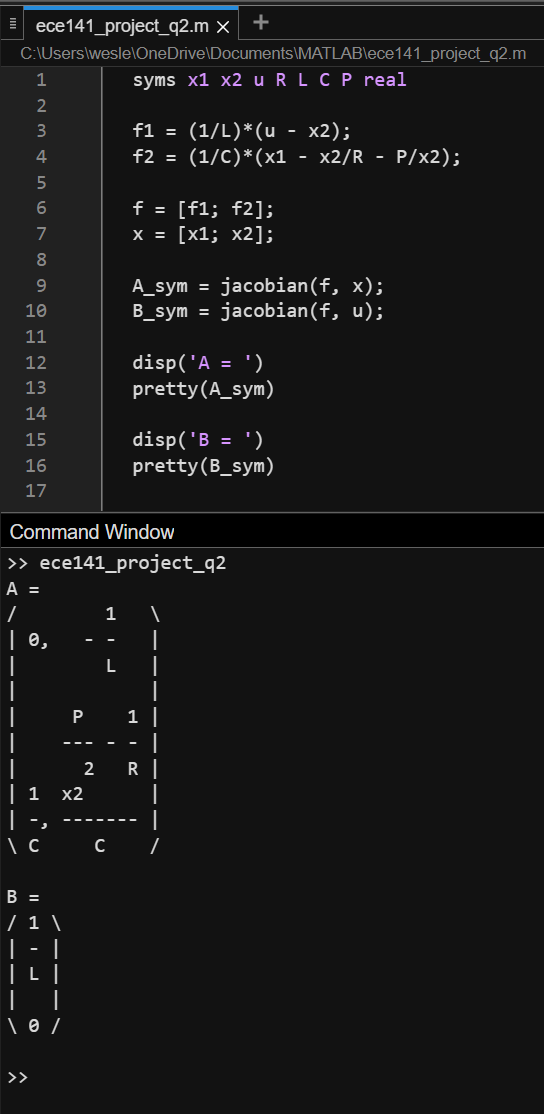
\includegraphics[width = \textwidth]{matlab2.png}
  \end{minipage}\hfill
  \begin{minipage}[t]{0.4\textwidth}
    \vspace{5pt}
    \textbf{Code Snippet 2}:\\
    This MATLAB script shows the definition of the variables $x_1, x_2, u, R, L, C, P$, as seen in Part 1.\\ 

    We then construct the matrices $f$ and $x$. $f$ is the state space representation of the system and $x$ is defined to be the state space variables.\\

    The matrices $A$ and $B$ are then defined as the Jacobian of $f$ with respect to $x$ and $u$, respectively.\\

    \begin{tcolorbox}[enhanced, frame hidden, colback=white, borderline west={1pt}{0pt}{gray}]
      The matrix $A$ is defined to be the State Matrix that defines the changes to the internal state dynamics.\\

      The matrix $B$ is defined to be the Input Matrix that defines how inputs affect states.
    \end{tcolorbox}

    The matrices are then displayed on Matlab script. \\The displayed matrices match our calculated matrix values.
  \end{minipage}
\end{tcolorbox}
\newpage

\section{Open Loop Transfer Function}
Find the open-loop transfer function $H(s)$ from input $\delta v_s$ to output $\delta v_{dc}$ in s-domain, assuming zero initial conditions. Find the relationship between R, L, C, and P that would ensure the linearized system would remain stable.

\

\begin{tcolorbox}[enhanced, frame hidden, colback=white, borderline west={1pt}{0pt}{gray}]
  \large{Transfer Function}\\
  \normalsize{}
  \begin{align*}
    \text{Linear System TF} & \ & H(s) &= \dfrac{\delta v_{dc}(s)}{\delta v_s(s)}\\
    \text{Using:} & \ & H(s) &= C(sI - A)^{-1}B\\
    \text{Where:} & \ & C_{out} &= \begin{bmatrix}0&1\end{bmatrix} 
  \end{align*}
  This concludes to be a second order transfer function.
\end{tcolorbox}

\

\begin{tcolorbox}[enhanced, frame hidden, colback=white, borderline west={1pt}{0pt}{gray}]
  \begin{minipage}[t]{0.45\textwidth}
    \vspace{0pt}
    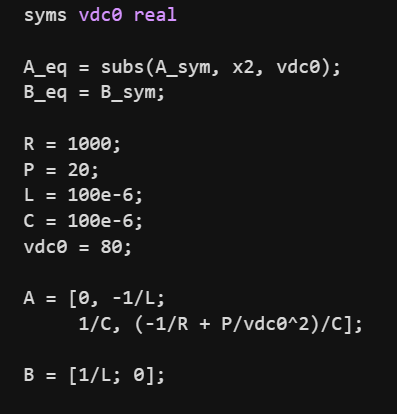
\includegraphics[width = \textwidth]{matlab3.png}
  \end{minipage}\hfill
  \begin{minipage}[t]{0.45\textwidth}
    \vspace{5pt}
    \textbf{Code Snippet 3}:
    This MATLAB script shows the initialization of the variables $R, P, L, C$, and $v_{dc0}$ so that the following transfer function code will compile. Matlab requires real number values.\\
    
    These variables are fetched from the project spec. 
  \end{minipage}
\end{tcolorbox}

\

\begin{tcolorbox}[enhanced, frame hidden, colback=white, borderline west={1pt}{0pt}{gray}]
  \begin{minipage}[t]{0.5\textwidth}
    \vspace{0pt}
    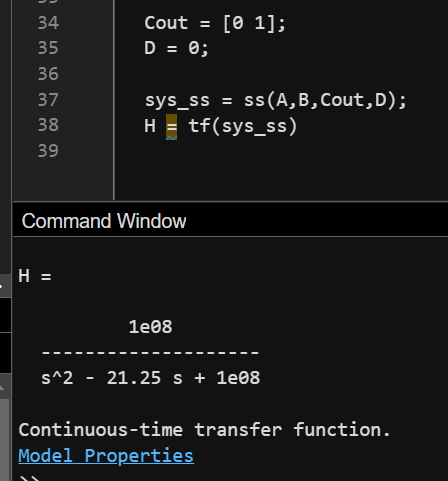
\includegraphics[width = \textwidth]{matlab4.png}
  \end{minipage}\hfill
  \begin{minipage}[t]{0.4\textwidth}
    \vspace{5pt}
    \textbf{Code Snippet 4}:
    This MATLAB script shows the initialization of the matrices $C$ and $D$ and calculates the transfer function from all four state-space matrices.\\

    The matrix $C$ maps the states to the output. It describes what part of the internal system states you observe.\\

    The matrix $D$ maps the input directly to the output. It describes any instantaneous effects of the input on the output.\\
  \end{minipage}
\end{tcolorbox}

\

\begin{tcolorbox}[enhanced, frame hidden, colback=white, borderline west={1pt}{0pt}{gray}]
  \large{Calculated Transfer Function}
  \normalsize{}
  From the Matlab simulation: \\
  \[
    \boxed{
      H(s) = \dfrac{10^8}{s^2 -21.25s+10^8}
    }
  \]
\end{tcolorbox}

\

\begin{tcolorbox}[enhanced, frame hidden, colback=white, borderline west={1pt}{0pt}{gray}]
  \large{Stability}\\
  \normalsize{}
  For a 2nd order system, stability requires that:\\
  $\hookrightarrow$ trace$(A) < 0$\\
  $\hookrightarrow$ det$(A) > 0$
  \begin{tcolorbox}[enhanced, frame hidden, colback=white, borderline west={1pt}{0pt}{gray}]
    \textbf{Trace}\\
    \begin{align*}
      tr(A) &= \dfrac{1}{C}(-\dfrac{1}{R}+\dfrac{P}{v^2_{dc0}})\\
      \dfrac{1}{C}&(-\dfrac{1}{R}+\dfrac{P}{v^2_{dc0}}) < 0 & \text{need to be negative trace}\\
      &-\dfrac{1}{R}+\dfrac{P}{v^2_{dc0}} < 0 & \text{since } C > 0\\
      &\dfrac{P}{v^2_{dc0}} < \dfrac{1}{R}\\
      &P < \dfrac{v^2_{dc0}}{R}\\
    \end{align*}
  \end{tcolorbox}
  \begin{tcolorbox}[enhanced, frame hidden, colback=white, borderline west={1pt}{0pt}{gray}]
    \textbf{Determinant}\\

    det$(A) = \dfrac{1}{LC} > 0$\\

    which is already true, since $L, C > 0$.
  \end{tcolorbox}


  \[
    \boxed{
      \dfrac{P}{v^2_{dc0}} < \dfrac{1}{R}
    }
  \]
  Constant power loads behave like negative resistance. \\
  Too much power would make the system unstable.
\end{tcolorbox}

\

\section{Equilibrium Values for the Current through the Wire}
Assume the parallel resistance of $R = 1000\Omega$, the CPL power constant of $P = 20W$ and, input equilibrium DC voltage of $v_{s0} = 80V$. Find all possible corresponding equilibrium values for the current through the wire and the voltage across the outdoor converter (i.e., $i_{l0}$ and $v_{dc_0}$ respectively.)\\

\textbf{Goal: }Find the equilibrium values for the current through the wire and the voltage across the outdoor converter.\\

\textbf{Given values: }$R = 1000\Omega$, $P = 20W$, $v_{s0} = 80V$. \\
$\hookrightarrow$ At equilibrium, $\dot{x_1} = 0$, $\dot{x_2} = 0$.

\

\begin{tcolorbox}[enhanced, frame hidden, colback=white, borderline west={1pt}{0pt}{gray}]
  \large{From inductor equation}
  \normalsize{}
  \begin{align*}
    0 &= \dfrac{1}{L}(v_{s0} - v_{dc0})\\
    v_{dc0} = v_{s0} &= 80V
  \end{align*}


  \large{From capacitor equation}
  \normalsize{}
  \begin{align*}
    0 &= i_{l0} - \dfrac{v_{dc0}}{R} - \dfrac{P}{v_{dc0}}\\
    i_{l0} &= \dfrac{v_{dc0}}{R} + \dfrac{P}{v_{dc0}}\\
  \end{align*}
  Resistor current: 80/1000 = 0.08A.\\
  CPL current: 20/80 = 0.25A.\\
  \begin{align*}
    i_{l0} &= 0.08A + 0.25A = 0.33A
  \end{align*}

  Thus, \[
  \boxed{i_{l0} = 0.33A} 
  \]
  
\end{tcolorbox}

\

\begin{tcolorbox}[enhanced, frame hidden, colback=white, borderline west={1pt}{0pt}{gray}]
  \begin{minipage}[t]{0.5\textwidth}
    \vspace{0pt}
    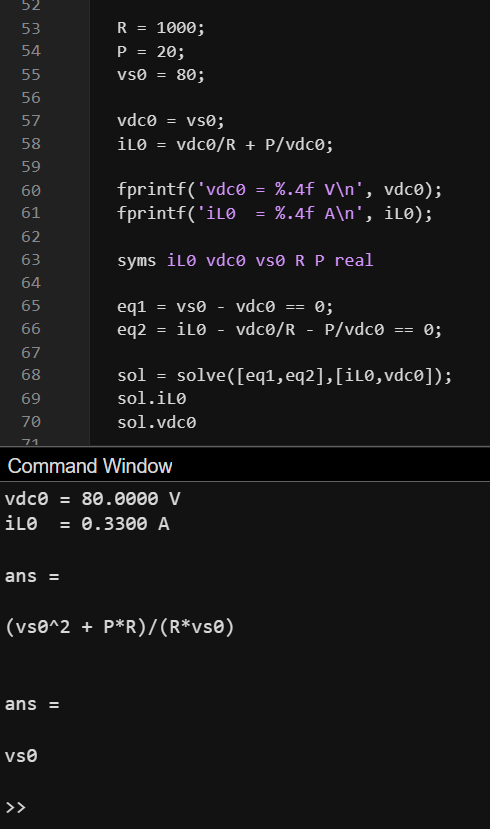
\includegraphics[width = \textwidth]{matlab5.png}
  \end{minipage}\hfill
  \begin{minipage}[t]{0.45\textwidth}
    \vspace{5pt}
    \textbf{Code Snippet 5}:
    Using the given values: $R = 1000\Omega, P = 20W, v_{s0} = 80V$, the Matlab script uses the previous inductor and capacitor $KVL/KCL$ equations to solve for the capacitor voltage ($v_{dc0}$) and the inductor current ($i_l$).\\

    As expected, the solved values of $v_{dc0}$ and $i_l0$ match our calculated values: $80V$ and $0.33A$ respectively.
  \end{minipage}
\end{tcolorbox}

\

\section{Stability}
Consider the system linearized around the equilibrium point with thw \textit{lowest} possible value you obtained for $v_{dc_0}$ in Part 4. Assume the same values for R and P as in Part 4 with the addition of $C = 100\mu F$ and $L = 100\mu H$. Is this linearized system BIBO stable? Recall Part 3.\\

\textbf{Goal: }Checking if the linearized system around the lowest equilibrium point is BIBO stable.\\

\textbf{Given: }$C = 100\mu F$, $L = 100\mu H$

\

\begin{tcolorbox}[enhanced, frame hidden, colback=white, borderline west={1pt}{0pt}{gray}]
  Condition from Part 3: $\dfrac{P}{v^2_{dc0}} < \dfrac{1}{R}$
\end{tcolorbox}

\

\begin{tcolorbox}[enhanced, frame hidden, colback=white, borderline west={1pt}{0pt}{gray}]
  Computing this inequality using:\\
  $\hookrightarrow P = 20W$\\
  $\hookrightarrow v^2_{dc0} = 80V$\\
  $\hookrightarrow R = 1000\Omega$\\

  LHS: $\dfrac{P}{v^2_{dc0}} = \dfrac{20}{80^2} = 0.003125$\\

  RHS: $\dfrac{1}{R} = \dfrac{1}{1000} = 0.001$\\

  Since $0.003125 > 0.001$, the system becomes \textbf{unstable}.

  \begin{tcolorbox}[enhanced, frame hidden, colback=white, borderline west={1pt}{0pt}{gray}]
    \textbf{Using trace:}\\
    Plugging in the values into the matrix \textbf{A}: $L = 100 * 10^{-6}, C = 100 * 10^{-6}, v_{dc0} = 80$\\

    \begin{align*}
      \text{\textbf{A}} &= \begin{bmatrix}
        0 & -10000\\
        10000 & \dfrac{-1/1000 + 20/80^2}{100*10^{-6}}\\
      \end{bmatrix}\\
      \text{\textbf{A}} &= \begin{bmatrix}
        0 & -10000\\
        10000 & 21.25\\
      \end{bmatrix}
    \end{align*}

    tr$(A)$ = $0 + 21.25 = 21.25 > 0$\\

    Since tr$(A) > 0$, the system becomes \textbf{unstable}.
  \end{tcolorbox}

  Thus, the linearized system is \textbf{not BIBO stable}.\\
  The system's poles are not both in the left-half plane. The stability condition defined in Part 3 is violated. \\

  Thus, the \textit{CPL} destabilizes the system.\\
\end{tcolorbox}

\

\begin{tcolorbox}[enhanced, frame hidden, colback=white, borderline west={1pt}{0pt}{gray}]
  \begin{minipage}[t]{0.5\textwidth}
    \vspace{0pt}
    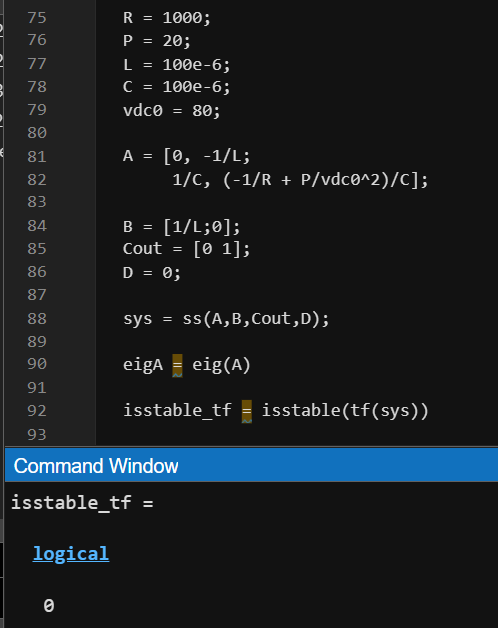
\includegraphics[width = \textwidth]{matlab6.png}
  \end{minipage}\hfill
  \begin{minipage}[t]{0.45\textwidth}
    \vspace{5pt}
    \textbf{Code Snippet 6}:\\
    This Matlab script takes in the values for $R, P, L, C$, and $v_{dc0}$, redefines the matrices ($\textbf{A, B, C, D}$), defines the eigenvector of $\textbf{A}$, and lastly, solves if the system as a whole is stable.\\

    The results in the command window show that the system is in fact \textbf{unstable}.
  \end{minipage}
\end{tcolorbox}

\

\section{Controller Design}
Consider the same linearized system as in Part 5, with all the same values. Let $y = \delta x_2$. Recall the open-loop transfer function $H$. Build the linearized model in Simulink. Use a solver for stiff differential equations (e.g., ode23s) when using Simulink. Design a controller such that the closed-loop system's output decays to 0 in no more than 0.05s with no overshoot and the initial conditions of $\delta x(0) = [8 \;\; -8]$. 

\

\textbf{Goal: }Design a controller such that the output decays to 0 in 0.05 seconds or less. There shall be no overshoot. \\

\textbf{Given specs: }\\
$\hookrightarrow$ Settling time $\leq 0.05s$\\
$\hookrightarrow$ No overshoot\\
$\hookrightarrow$ Initial condition: \\

\hspace{0.05\textwidth} $\hookrightarrow \delta x(0) = \begin{bmatrix}
  8\\-8\\
\end{bmatrix}$

Letting $y = \delta x_2$\\

The system is disturbed from equilibrium and the goal is to make the output return to zero quickly and smoothly.

\begin{tcolorbox}[enhanced, frame hidden, colback=white, borderline west={1pt}{0pt}{gray}]
  \large{Restating Values}
  \normalsize{}
  \begin{tcolorbox}[enhanced, frame hidden, colback=white, borderline west={1pt}{0pt}{gray}]
    Matrices: $\textbf{A} = \begin{bmatrix}
      0 & -\dfrac{1}{L}\\
      \dfrac{1}{C} & \dfrac{1}{C}(-\dfrac{1}{R} + \dfrac{P}{v^2_{dc0}})
    \end{bmatrix}$, $\textbf{B} = \begin{bmatrix}
      \dfrac{1}{L}\\
      0
    \end{bmatrix}$
  \end{tcolorbox}
  \begin{tcolorbox}[enhanced, frame hidden, colback=white, borderline west={1pt}{0pt}{gray}]
    Circuit values: $R = 1000\Omega, P = 20W, L = 100\mu H, C = 100\mu F, v_{dc0} = 80V$
  \end{tcolorbox}
  \begin{tcolorbox}[enhanced, frame hidden, colback=white, borderline west={1pt}{0pt}{gray}]
    $\dfrac{1}{L} = 10000$, $\dfrac{1}{C} = 10000$.\\

    $\dfrac{1}{C}(-\dfrac{1}{R} + \dfrac{P}{v^2_{dc0}}) = \dfrac{1}{100 * 10^{-6}}(-0.001 + \dfrac{20}{80^2}) = 21.25$
  \end{tcolorbox} 
  \begin{tcolorbox}[enhanced, frame hidden, colback=white, borderline west={1pt}{0pt}{gray}]
    Therefore, $\textbf{A} = \begin{bmatrix}
      0 & -10000\\
      10000 & 21.25\\
    \end{bmatrix}$, $\textbf{B} = \begin{bmatrix}
      10000\\
      0
    \end{bmatrix}$
  \end{tcolorbox} 
  \begin{tcolorbox}[enhanced, frame hidden, colback=white, borderline west={1pt}{0pt}{gray}]
    The output is stated to be: $y = \delta x_2$.\\

    So, $C_{out} = \begin{bmatrix}
      0&1
    \end{bmatrix}$, $D = 0$
  \end{tcolorbox} 
\end{tcolorbox} 

\

\begin{tcolorbox}[enhanced, frame hidden, colback=white, borderline west={1pt}{0pt}{gray}]
  \large{Transfer Function}\\
  \normalsize{}
  From the linearized state-space model, the transfer function from $\delta v_s$ to $\delta v_{dc}$ is \\
  \[
    \centering
    H(s) = \dfrac{\delta v_{dc}(s)}{\delta v_s(s)}
  \]
  We found that the transfer function becomes:\\
  \[
    \centering
    H(s) = \dfrac{10^8}{s^2 - 21.25s + 10^8}
  \]
  The denominator ($s^2 - 21.25s + 10^8$) has a negative coefficient, which shows that the system is \underline{unstable}, since all of the coefficients in the denominator of the transfer function of a system must be positive. 
\end{tcolorbox}

\

\begin{tcolorbox}[enhanced, frame hidden, colback=white, borderline west={1pt}{0pt}{gray}]
  \large{Why a plain proportional controller is not enough}
  \normalsize{}
  \[C(s) = K_p\]
  $\hookrightarrow$ trying a proportional (P) controller $C(s)$.\\

  The closed-loop characteristic equation becomes 
  \[
  1 + K_p H(s) = 0
  \]
  \[
  s^2 - 21.25s + 10^8(1+K_p)
  \]
  The $"-21.25s"$ term still contains a negative coefficient.\\
  Thus, we may not use a proportional controller, since this controller cannot fix the unstable damping term. \\
  
  In other words, \textbf{P} only is not enough. We must use a controller that change the s-coefficient, using derivative action or a lead compensator.
\end{tcolorbox}

\

\begin{tcolorbox}[enhanced, frame hidden, colback=white, borderline west={1pt}{0pt}{gray}]
  \large{PD Controller}\\
  \normalsize{}
  Using a PD controller:
  \[C(s) = K_p + K_ds\]
  equivalent to PID with $K_i = 0$\\

  Characteristic Polynomial becomes: 
  \[s^2 + (10^8 K_d -21.25)s + 10^8 (1+K_p)\]
  This can potentially get rid of the negative coefficient in the controller to make it stable. Now, the coefficient $10^8 K_d -21.25$ must be positive. Since we introduced $K_p$ as well, the final term: $10^8(1 + K_p)$ must be positive as well.\\

  Since we do not want overshoot, the closed-loop poles must be real and negative, perfectly well damped. Choose two real poles $p_1, p_2$.\\
  \[T_s \approx \dfrac{4}{|pole|}\]
  \[T_s \leq 0.05\]
  $\hookrightarrow$ thus, $|pole| \geq 80$.
\end{tcolorbox}

\

\begin{tcolorbox}[enhanced, frame hidden, colback=white, borderline west={1pt}{0pt}{gray}]
  An option is to use a PD controller to make the system overdamped, so that guarantees no overshoot.\\
  \begin{tcolorbox}[enhanced, frame hidden, colback=white, borderline west={1pt}{0pt}{gray}]
    Assuming $K_p = 0$ since the last term will always be positive, we then calculate the $K_d$ needed
    to make this system overdamped.
    \begin{align*}
      D &= b^2-4ac>0\\
      D &= (10^8 K_d -21.25)^2 -4*10^8 > 0\\
      (10^8 K_d -21.25)^2 &>4*10^8 \\
      10^8 K_d -21.25 &>2*10^4 \\
      K_d * 10^8 &> \approx 2*10^4\\
      K_d &> 2*10^{-4}\\
    \end{align*}
    $\hookrightarrow$ thus, this criterion of $K_d$ makes the 2nd order controller overdamped.
  \end{tcolorbox}
  
  \begin{tcolorbox}[enhanced, frame hidden, colback=white, borderline west={1pt}{0pt}{gray}]
    To ensure that the system is stable, all of the coefficients in the 2nd
    order system characteristic polynomial equation must be positive.
    \begin{align*}
      10^8K_d -21.25 &> 0\\
      10^8(1+K_p) &> 0\\
    \end{align*}
    \[K_d > 2.125 *10^{-7}, K_p >\approx 0\]
    $\hookrightarrow$ thus, with the coefficients all positive, the system is ensured to be stable.
  \end{tcolorbox}
  
  An example of controller values are $K_p = 0$, $K_d = 2.5*10^{-4}$.\\
  This yields a polynomial equation of:
  \[s^2 + 24978.75s+10^8\]
  $\hookrightarrow s \approx -19971.65, -5007.10$, both negative and makes a system stable. It also decays extremely fast. It is a very strong set of poles.
  \[T_s \approx \dfrac{4}{5007} \approx 0.0008s \leq 0.05s\]
\end{tcolorbox}

\

\begin{tcolorbox}[enhanced, frame hidden, colback=white, borderline west={1pt}{0pt}{gray}]
  \begin{minipage}[t]{0.55\textwidth}
    \vspace{0pt}
    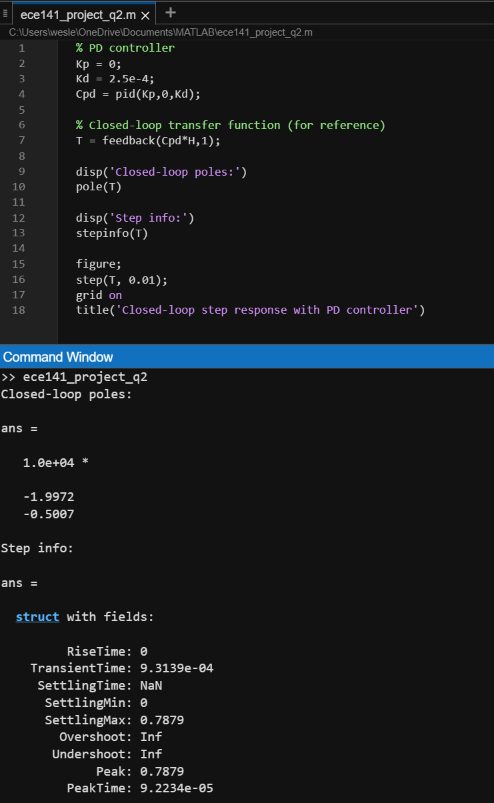
\includegraphics[width = \textwidth]{matlab7.png}
  \end{minipage}\hfill
  \begin{minipage}[t]{0.4\textwidth}
    \vspace{0pt}
    \textbf{Code Snippet 7: }In this Matlab code snippet, the closed loop poles were calculated from the original controller constants $K_p$ and $K_d$. 
    The poles are equivalent to the values that were calculated earlier. 
    The step info were also calculated in Matlab and analyzing the transient time, it is much less than the specified 0.005s maximum. 
    The transient time is calculated to be 0.00093s. 
  \end{minipage}
\end{tcolorbox}

\

\begin{tcolorbox}[enhanced, frame hidden, colback=white, borderline west={1pt}{0pt}{gray}]
  \begin{minipage}{0.80\textwidth}
    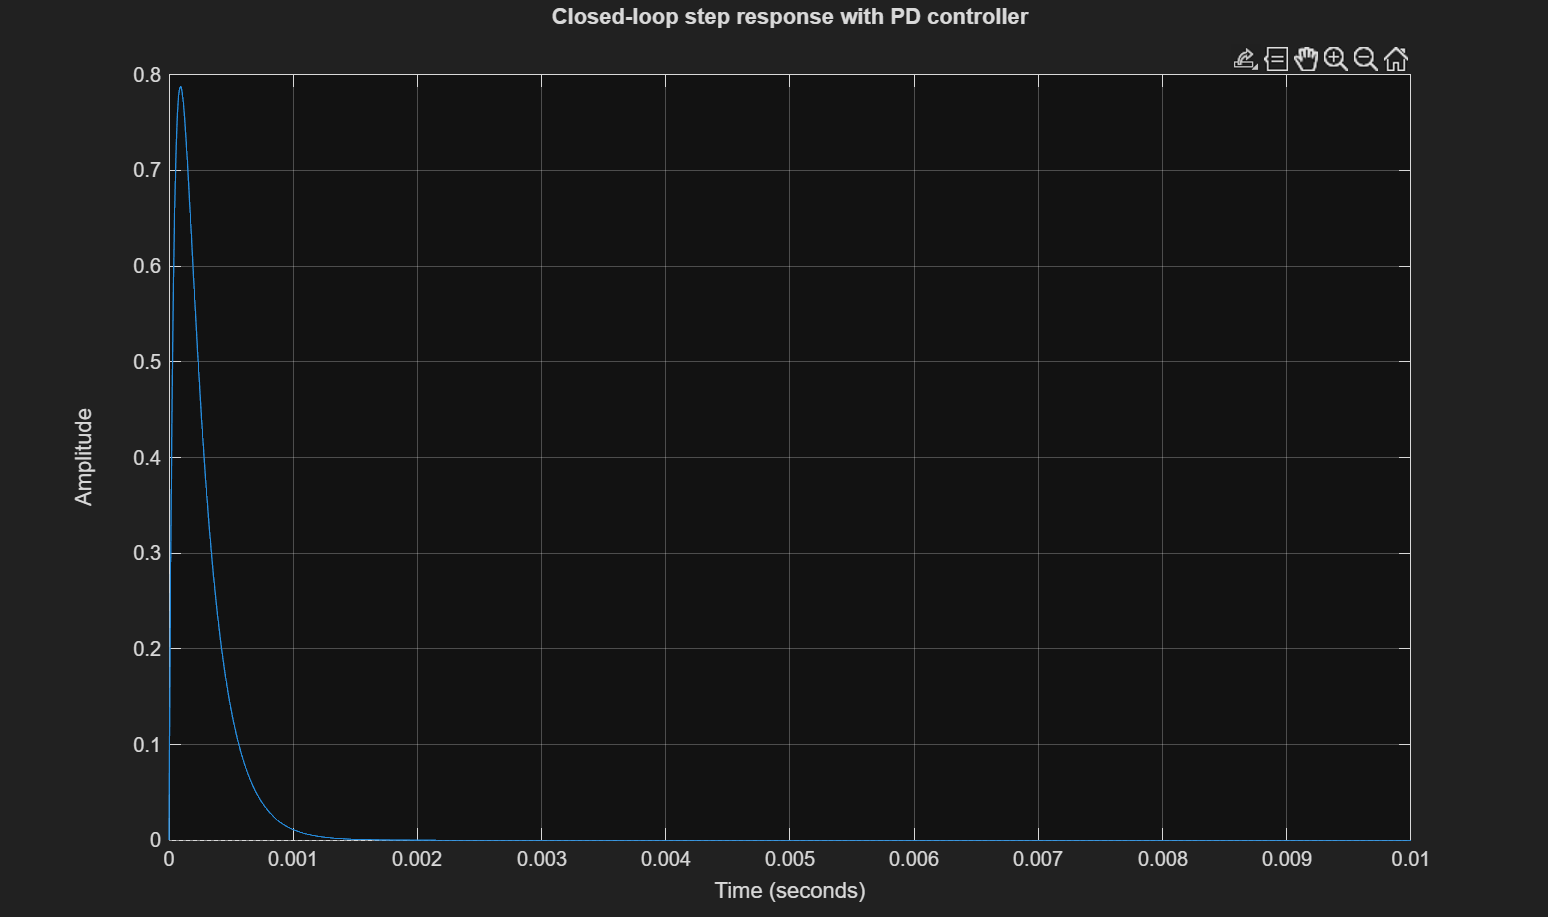
\includegraphics[width = \textwidth]{figure1.png}\\
  \end{minipage}\\
  \textbf{Figure 1: }This figure represents the closed-loop step response with a PD controller with the given specifications above. \\
  In this figure, it is shown that the system experiences a disturbance at time = 0 seconds. \\
  Then, the controller brings it back down to 0 within the 0.005s specification requirement.
\end{tcolorbox}

\

\begin{tcolorbox}[enhanced, frame hidden, colback=white, borderline west={1pt}{0pt}{gray}]
  \begin{minipage}{0.80\textwidth}
    \vspace{-30pt}
    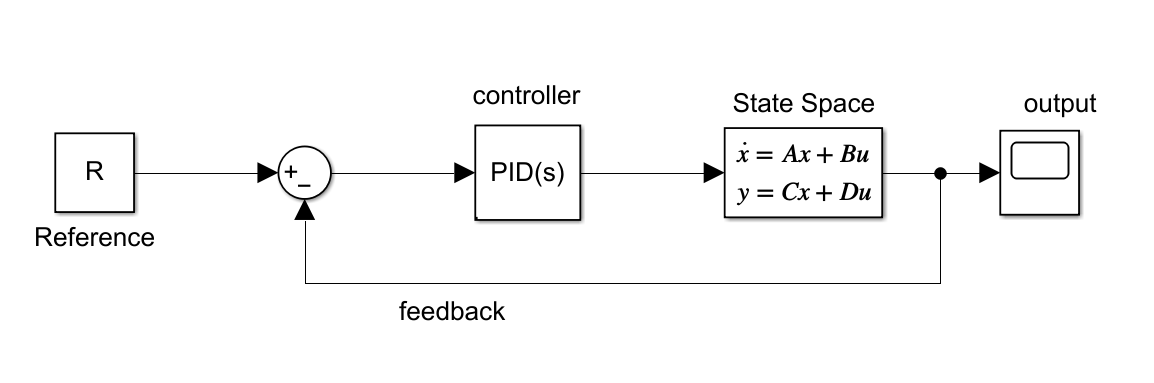
\includegraphics[width = \textwidth]{figure2.png}\\
  \end{minipage}\\
  \textbf{Figure 2: }This figure represents the complete block diagram of the system. It highlights the reference input, the PID controller that we are designing, the state spaces, and the feedback and ultimately, the output.
  The state space block takes the previous values for the matrices of 
  \textbf{A}, \textbf{B}, \textbf{C}, and \textbf{D}.\\

  The system also uses the initial condition $\begin{bmatrix}
    8 & -8
  \end{bmatrix}$;
\end{tcolorbox}

\

\begin{tcolorbox}[enhanced, frame hidden, colback=white, borderline west={1pt}{0pt}{gray}]
  \begin{minipage}{0.80\textwidth}
    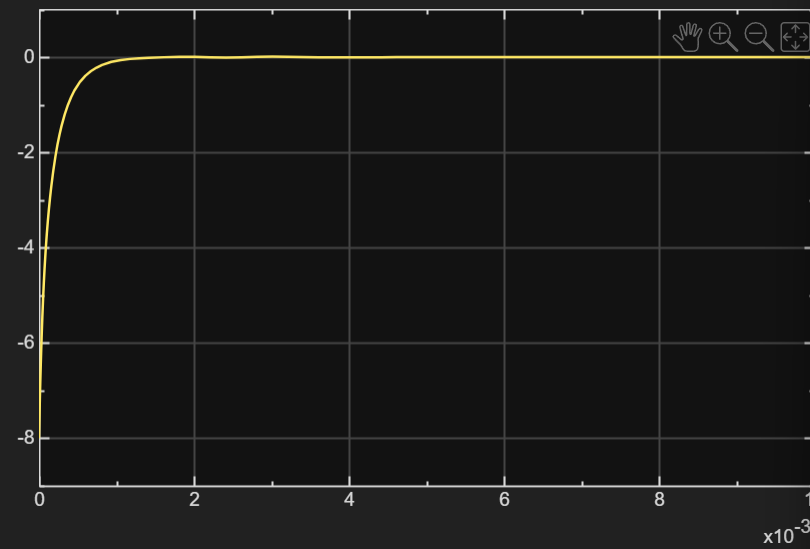
\includegraphics[width = \textwidth]{figure3.png}\\
  \end{minipage}\\
  \textbf{Figure 3: }This figure is the graph of the output of the entire system due to a disturbance.
  The disturbance is modeled as the initial condition as $\begin{bmatrix}
    8 & -8
  \end{bmatrix}$. 
  The PD controller uses the values:
  \[K_p = 0, K_i = 0, K_d = 2.5*10^{-4}\]
  designed so that the controller is overdamped, specifically to bring the 
  output value back down to 0 as fast as possible with the least amount of 
  oscillation. As seen in Figure 3, we see that the settling time is 
  way below the specified settling time of 0.05s.
\end{tcolorbox}

\

\begin{tcolorbox}[enhanced, frame hidden, colback=white, borderline west={1pt}{0pt}{gray}]
  
\end{tcolorbox}

\section{Simulink Implementation} 
Implement the original nonlinear model in Simulink, assuming the initial states of $x(0) = x_0 + \delta x(0)$ and with the same parameters as Part 6. Keep in mind that the input $v_s$ and the states $v_{dc}$ needs to be non-negative at all times, with the additional safety requirement that they shall not exceed $160V, 20A and 200V$ respectively. \textit{Hint: } you can use a saturation block in Simulink and set its lower and upper limits to the corresponding safety bounds. Apply the controller found in Part 6 by placing it in the closed-loop with the nonlinear model in Simulink. Since we are translating the system back to the original system, adjust the controller input appropriately, and the output's settling value. If needed, redesign your controller. Comment on the differences you observe as you implement the controller in the linearized vs the nonlinear model.

\

\begin{tcolorbox}[enhanced, frame hidden, colback=white, borderline west={1pt}{0pt}{gray}]
  
\end{tcolorbox}

\

\begin{tcolorbox}[enhanced, frame hidden, colback=white, borderline west={1pt}{0pt}{gray}]
  
\end{tcolorbox}

\

\begin{tcolorbox}[enhanced, frame hidden, colback=white, borderline west={1pt}{0pt}{gray}]
  
\end{tcolorbox}

\

\begin{tcolorbox}[enhanced, frame hidden, colback=white, borderline west={1pt}{0pt}{gray}]
  
\end{tcolorbox}

\

\begin{tcolorbox}[enhanced, frame hidden, colback=white, borderline west={1pt}{0pt}{gray}]
  
\end{tcolorbox}

\

\begin{tcolorbox}[enhanced, frame hidden, colback=white, borderline west={1pt}{0pt}{gray}]
  
\end{tcolorbox}

\

\begin{tcolorbox}[enhanced, frame hidden, colback=white, borderline west={1pt}{0pt}{gray}]
  
\end{tcolorbox}

\

\begin{tcolorbox}[enhanced, frame hidden, colback=white, borderline west={1pt}{0pt}{gray}]
  
\end{tcolorbox}
\end{document}